\documentclass{IEEEcsmag}

\usepackage[colorlinks,urlcolor=blue,linkcolor=blue,citecolor=blue]{hyperref}

\usepackage{upmath}
\usepackage{amssymb}
\usepackage{amsmath}
\usepackage{array}
\newcolumntype{P}[1]{>{\centering\arraybackslash}p{#1}}

\jvol{XX}
\jnum{XX}
\paper{8}
\jmonth{May/June}
\jname{Computing in Science and Engineering}
\pubyear{2021}
\newtheorem{theorem}{Theorem}
\newtheorem{lemma}{Lemma}

\setcounter{secnumdepth}{0}

\begin{document}

\sptitle{Department: Head}
\editor{Editor: Name, xxxx@email}

\title{PyExaFMM: Designing a high-performance point fast multipole solver in Python with Numba}

\author{\ S. Kailasa}
\affil{\ Department of Mathematics, University College London}

\author{\ T. Betcke}
\affil{\ Department of Mathematics, University College London}

\author{\ T. Wang}
\affil{\ Department of Mechanical and Aerospace Engineering, The George Washington University}

\author{\ L. A. Barba}
\affil{\ Department of Mechanical and Aerospace Engineering, The George Washington University}

\markboth{Department Head}{Paper title}

\begin{abstract}
PyExaFMM was developed on the success of the ExaFMM project, and answer the question of whether it was possible to develop a high-performance scientific software without resorting to a lower level language. High-level languages are appealing, reducing the barrier to entry for potential contributors, as well as making deployment to new architectures or platforms easier. The FMM is a good case study for understanding the maturity of Python for developing high-performance software, due its reliance on a complex hierarchical tree data structure. In this article we explore the software engineering and mathematical techniques used to extract performance for PyExaFMM, and we report that we achieve runtimes within $\mathcal{O}(10)$ of the state of the art C++ implementation, with comparable accuracy, for three dimensional electrostatic problems in single precision.

\end{abstract}

\maketitle
\chapterinitial{We introduce PyExaFMM}, a Python-based solver for the point Fast Multipole Method [FMM], designed for high-performance computing [HPC]. The vision behind building a HPC library in Python is one where a domain specialist may be able to rapidly iterate to a high-performance application from a prototype, without necessarily having expertise in software development. Python has the additional benefit of simple cross platform build tools, such as Conda, making it easy for developers to code once and deploy everywhere. An FMM implementation is an excellent case study to understand the maturity of Python for HPC development. As Numba is built to optimize operations on arrays, it represents a challenge to develop efficient representations and operations for the tree on which the algorithm is based.

PyExaFMM is currently a single node implementation designed for three-dimensional problems, implementing parallel strategies on multicore architectures, similar to \cite{Bramas2020, Wang2021}. As with all Python applications, performance is degraded by portions of code that are unavoidably interpreted. However, this represents a compromise between usability and performance. Where by usability, we mean the ease by which non-software specialists can understand, alter, or extend the codebase to their needs. Using lines-of-code [LOC] as a rough metric of usability, PyExaFMM consists of approximately 5,800 LOC, compared with approximately 20,000 LOC and 50,000 LOC for the comparable C++ implementations,  TBFMM \cite{Bramas2020} and ExaFMM-T \cite{Wang2021} respectively.

In this article we begin by providing an overview of the FMM algorithm, as well as the Kernel-Independent FMM [KIFMM] variant
\cite{Ying2004} used by PyExaFMM. We proceed to introduce Numba, and discuss how it's used to accelerate computations. We continue by examining other mathematical and software based optimizations used to extract performance. Specifically, the efficient pre-computation, and application of various FMM operations, and an overview of the software's design. We conclude with a comparison of performance, in terms of accuracy, runtimes, and memory footprint, with the comparable state-of-the-art C++ implementation from the ExaFMM project, ExaFMM-T \cite{Wang2021}.

\section{FAST MULTIPOLE METHODS}

\subsection{The N-Body Problem}

The FMM \cite{Greengard1987}, approximates the solution of the so called $N$ body problem, in which one seeks to calculate pairwise interactions between $N$ objects. This problem arises in numerous contexts in science and engineering, for example in the calculation of electrostatic or gravitational potentials due to a set of charged or massive source objects. This is an important calculation, as with an estimate of potential one is able to describe the corresponding electric, or gravitational field due to these objects, and hence the forces they exert. In this article we use the electrostatic potential generated by point charges in three dimensions as our model to explore the FMM. Here, the potential, $\phi(x_j)$, for a given point at position $x_j$, or `target', due to $N$ points at positions $x_i$, or `sources', where $i \in [1, ..., N]$, each with a charge $q_i$, can be written as,

\begin{eqnarray}
	\phi(x_j) = \sum_{i=1}^{N} K(x_i, x_j) q_i,
\label{eq:sec:intro:nbody_problem}
\end{eqnarray}


here $K(\cdot, \cdot)$ is called the Green's function, or kernel function. For electrostatic problems in three dimensions it is,

\begin{eqnarray}
	K(x, y) = \frac{1}{4\epsilon_0\pi|x-y|},
\label{eq:sec:intro:laplace_kernel}
\end{eqnarray}

where $\epsilon_0$ is the permittivity of free space, and is referred to as the Laplace kernel. Without loss of generality, we consider the set of sources and set of targets to correspond to the same set of points.

Intuitively, (\ref{eq:sec:intro:laplace_kernel}) can be understood as encoding a `decay' relationship between two given points. The closer they are the higher their proportionate effect on each other's potential. Attempting to evaluate the sum in (\ref{eq:sec:intro:nbody_problem}) directly for $N$ points, results in algorithm of $\mathcal{O}(N^2)$ runtime complexity, as the sum will have to be repeated $N$ times. However the FMM is able to approximate (\ref{eq:sec:intro:nbody_problem}) with just $\mathcal{O}(N)$ runtime complexity, with proscribed error bounds. This makes the simulation of granular physically realistic systems tractable.

\subsection{The FMM Algorithm}\label{sec:intro:algorithm}

The key idea behind the FMM is to encode the potential in the far field due to a cluster of points with a representative analytic series expansion centered on the cluster, referred to as a \textit{multipole expansion}. This expansion can be truncated to tune for a desired accuracy, which allows one to approximate the sum in (\ref{eq:sec:intro:nbody_problem}) with fewer calculations. Alternatively, we can center the expansion far away from the cluster, the encoded potentials are then referred to as a \textit{local expansion}. Translations between multipole and local expansions can be done analytically, and are critical in the development of the $\mathcal{O}(N)$ algorithm. However, this approximation is only valid where the kernel function of a problem exhibits appropriate `decay' characteristics, allowing us to assume that potential due to clusters of points far away from a region of interest can be approximated with a truncated representative expansion.

In the FMM, the problem domain is described by a cubic box enclosing all targets and sources, which is hierarchically partitioned into a structure known as a quadtree in two dimensions, and an octree in three dimensions. The partitioning is done recursively. Initially it is partitioned into four equal parts in two dimensions (eight in three dimensions), known as its children. Correspondingly the unrefined box is referred to as their parent. The children are each subsequently refined in a similar fashion. The final tree consisting of a series of hierarchically nested boxes.

The size of the box is described by its `level', with level zero denoting the unrefined box, level one denoting the level of its children, and so forth. One can define the maximum level of refinement through a parameter dictating the maximum allowable number of points contained within the finest box covering a portion of the domain. These finest boxes that remain after refinement are known as leaves. Note that the set of all leaves cover the entire domain, without overlap. One can choose to refine \textit{adaptively}, such that the leaves may be of different sizes, reflective of the underlying point distribution, or \textit{non-adaptively}, such that the leaves are all of a uniform size.

The FMM then consists of two sequential traversals of this tree, where boxes are considered level by level. Initially, during the \textit{upward pass}, multipole expansions for points contained in boxes at the leaf level are formed. This is referred to as the \textit{point-to-multipole} [P2M] operation. In order to obtain the multipole expansions for their parents, the expansion centers of a given box's children are shifted to the center of their shared parent box, and their coefficients are summed. This is referred to as the \textit{multipole-to-multipole} [M2M] operation. This is repeated bottom-up, level by level, until one is left with the multipole expansions of all boxes in the tree.

Subsequently, during the \textit{downward pass}, the multipole expansions of non-adjacent boxes of a given box are defined as being in its far field. In order to evaluate their contribution towards the potential for points within a given box, one translates their multipole expansion to a local expansion centered at the given box. This is referred to as the \textit{multipole-to-local} [M2L] operation. The local expansion is then transferred to the children of the given box by shifting the expansion center to the center of the child boxes, and updating the coefficients of the child boxes' local expansions. Proceeding top-down, considering boxes level by level, one is left with the local expansions for each leaf box. These are referred to as \textit{local-to-local} [L2L] operations.

Crucially the extent of the far field not already encapsulated in the local expansion shrinks as we descend down the levels of the tree. This is because the far field of a box's parent is already captured in the child's local expansion. These local expansions compress all of the contribution from the far field towards the potential for targets within a given leaf. Therefore the far field's effect on the potential of targets within a leaf box is entirely described by the local expansion.

The evaluation of the local expansion at the target points in a given leaf box is known as the \textit{local-to-point} [L2P] operation. Finally, the near fields of a given leaf box are evaluated directly using (\ref{eq:sec:intro:nbody_problem}), this is referred to as the \textit{point-to-point} [P2P] operation. As there are a fixed number of points per leaf node, the complexity of this direct evaluation is bounded. The operations in this scheme are illustrated for a two dimensional problem, with a uniform quadtree, in figure (\ref{fig:tree_traversal}).

% Larger figure
\begin{figure*}
\centerline{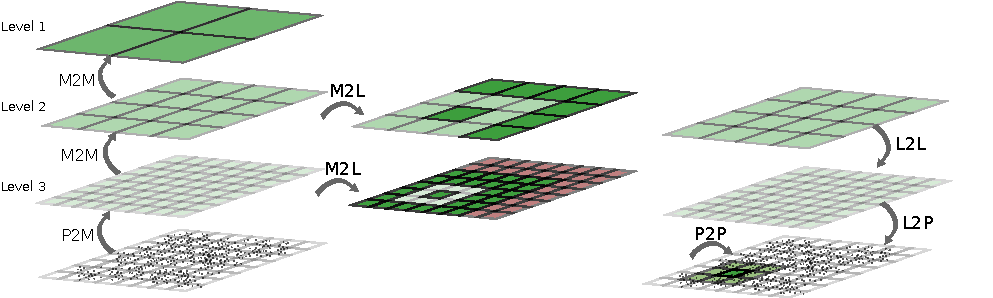
\includegraphics {figures/algorithm.pdf}}
\caption{The FMM illustrated for a two dimensional problem with a uniform quadtree. The left column illustrates the first two steps of the upward pass, beginning with the P2M operation to find the multipole expansions at the leaf level, followed by an M2M operation. The central and right columns illustrate the downward pass. In the central column, the far-field of a given box is highlighted, we observe that at level three the far field highlighted in red is already encapsulated in the local expansion of the given box due to the L2L translation from its parent. In the right column we see how the algorithm concludes with a given box evaluating it's near field of adjacent boxes, directly via the P2P operation.}
\label{fig:tree_traversal}
\end{figure*}

The $\mathcal{O}(N)$ algorithmic runtime complexity can be roughly seen to be the result of the ability to exactly translate between the multipole and local expansion representations for all boxes deemed to be in the far field of a given box, as well as the recursive procedure of the FMM. As a result of this, each box must only consider its interaction with a constant number of other boxes. As there are $\mathcal{O}(N)$ boxes in a given tree, the entire algorithm can be seen to be bounded by a runtime complexity of $\mathcal{O}(N)$.

\subsection{The Kernel Independent FMM}

PyExaFMM utilizes the KIFMM, first presented by Ying et. al \cite{Ying2004}. This algorithm represents the multipole expansions due to a cluster of charges as set of equivalent charge densities supported on a surface enclosing the cluster. The fields generated by the charges are matched with an equivalent field generated by these equivalent densities via a least-squares fitting of the potential they generate at another surface in the far field. This method generalizes the FMM to non-oscillatory second-order elliptic partial differential equations with constant coefficients, for example the Laplace or Stokes equations. This includes many common problems, such as our model electrostatic problem.

Consider the P2M operation illustrated in figure (\ref{fig:operators}a). A cubic \textit{equivalent} surface, sharing the same center, $S_e$ is used to enclose a leaf from the tree containing set of points. It is discretized with evenly spaced quadrature points placed its faces, each of which supports an equivalent charge density. In order to find these equivalent densities, we match the potential generated by the points directly, $\phi_c$, calculated using (\ref{eq:sec:intro:nbody_problem}) with that generated by the equivalent densities at the \textit{check} surface, $S_c$, in the far field, also centered on the box, which encloses both the box and the corresponding equivalent surface. Using (\ref{eq:sec:intro:nbody_problem}) we find,

\begin{equation}
	\sum_{x_i \in S_e, x_j \in S_c} K(x_i, x_j)q_i = \phi_c
	\label{eq:sec:intro:kifmm:p2m1}
\end{equation}

where $x_i$ and $x_j$ are the quadrature points for the equivalent and check surfaces respectively, $q_i$ is the equivalent charge density supported at $x_i$. Written in matrix form, we can write the equivalent densities, $q_e$, as the solution of the following linear system,

\begin{flalign}
	K q_e = \phi_c \\
	q_e = K^{-1} \phi_c
	\label{eq:sec:intro:p2m2}
\end{flalign}

where $K$ denotes a matrix with elements,

\begin{equation}
	K_{i, j} = K(x_i, x_j), \> \> \> x_j \in S_c, \> \> x_i \in S_e
	\label{eq:sec:intro:kifmm:matrixelements}
\end{equation}

We identify these equivalent densities as a multipole expansion. The order of this expansion, $p$, is related to the number of the quadrature points, $n$,  by,

\begin{equation}
	n = 6(p-1)^2+2
	\label{eq:sec:intro:kifmm:nquads}
\end{equation}

Equation (\ref{eq:sec:intro:p2m2}) is in general ill-conditioned, therefore we use a truncated singular value decomposition [SVD] of $K$, to calculate a pseudo-inverse. We cut off components corresponding to singular values smaller than machine epsilon in single precision.

As shown in figure (\ref{fig:operators}a), the equivalent surface is enclosed by the check surface for the P2M operation. When this is the case we refer to the surfaces as the \textit{upward} equivalent and check surface respectively. We find that the ratio of the side-length of the upward equivalent and check surfaces with respect to the tree node as 1.05 and 1.90 work well in practice.

We perform a similar calculation for the M2M operation, illustrated in figure (\ref{fig:operators}b). Here the upward equivalent density of a child box, is matched to that of its parent,

\begin{equation}
	K_c q_e^{child} = K_p q_e ^{parent}
\end{equation}

where $K_c$ and $K_p$ are matrices with elements as defined by (\ref{eq:sec:intro:kifmm:matrixelements}), where $S_c$ and $S_e$ denote their relevant check and equivalent surfaces. To find the child's contribution to the parent's upward equivalent density, and hence multipole expansion, we solve,

\begin{equation}
	q_e^{parent} = K_p^{-1}K_c q_e^{child}
\end{equation}

we refer to $K_p^{-1}K_c$ as the \textit{M2M operator}, with four unique operators in two dimensions (eight in three dimensions) corresponding to all the children of a given box. To find the corresponding \textit{L2L operators} and \textit{M2L operators}, we simply repeat the procedure with the appropriate check and equivalent surfaces. For the L2L operation, the check surface is placed inside the equivalent surface. This reflects the region in which we expect the local expansion to valid. Here they are referred to as the \textit{downward} check and equivalent surfaces respectively. For the M2L operation (fig. \ref{fig:operators}d) the upward equivalent surface of the source box, is matched to the potential generated by the downward equivalent surface at the target box.

We choose the upward equivalent surface to correspond to the downward check surface, and the downward equivalent surface to correspond to the upward check surface, for a given level. We then notice that the quantity $K^{-1}$ in (\ref{eq:sec:intro:p2m2}) can be re-used in the calculation of the M2M operator, as well as the M2L operator. Additionally, the M2M and L2L operators remain the same for all boxes in the tree.

% Larger figure
\begin{figure*}
	\centerline{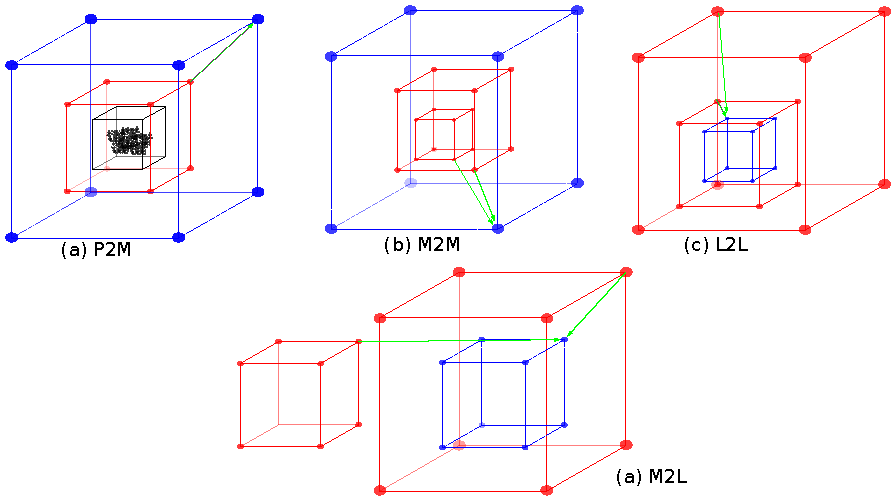
\includegraphics {figures/operators.pdf}}
	\caption{The operators of the KIFMM. Equivalent surfaces are denoted in red, check surfaces in blue, and the charged points are denoted in black. Surfaces are plotted with 8 quadrature points, for clarity.}
	\label{fig:operators}
\end{figure*}

As PyExaFMM uses adaptive octrees, there are further permutations in the composition of the near and far field we must describe. Consider a target box $T$, all source boxes $S$ directly neighboring $T$ (sharing an edge, face, or corner) are in $T$'s \textit{U list}. Denoting a neighbor of a box at the same level as its \textit{colleague}. The children of $T$'s colleagues which are not adjacent to $T$ are in its \textit{W list}, and the children of the colleagues of $T$'s parent which are not adjacent to $T$ are in its \textit{V list}. Finally, the \textit{X list} of T consists of boxes for which $T$ is in their W list. The X and W list are only calculated for leaf boxes. Collectively these lists are known as the \textit{interaction lists} of $T$, and are illustrated for a two dimensional problem in figure (\ref{fig:interaction_lists}).

Greater specification of the interaction lists allows for a more efficient algorithm implementation. Considering a source box in $T$'s W list, the multipole expansion of the source box is valid despite note being in $T$'s far field, therefore reducing the cost of calculating the near field contribution. For source boxes in $T$'s X list, the multipole expansion is not valid, as $T$ is not in the far-field of the source box. However, the source charges can be evaluated directly at the quadrature points on $T$'s downward equivalent surface. PyExaFMM also enforces a \textit{2:1 balance constraint} on the leaves, such that neighboring leaves may at most differ by one level. This constraint ensures small interaction lists, in the case of particle distributions with rapidly varying densities.

\begin{figure}
\centerline{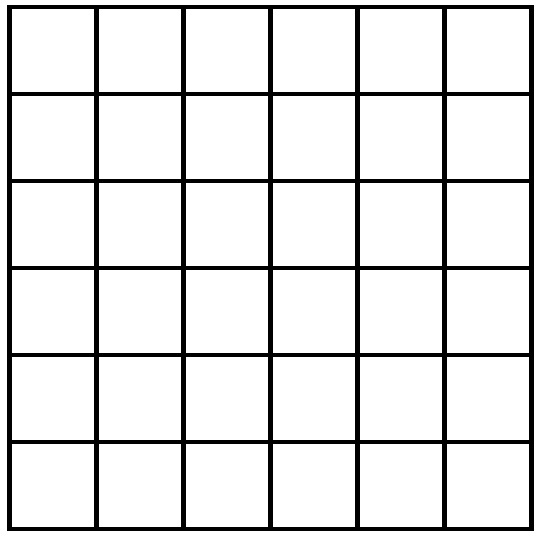
\includegraphics[width=18.5pc]{figures/interaction_lists.pdf}}
\caption{Interaction Lists for a target leaf box, $T$. Unmarked nodes are not considered to interact with $T$.}
\label{fig:interaction_lists}
\end{figure}

Implementing efficient KIFMMs relies on efficiently caching and loading the matrices that represent the P2M, M2M, L2L and M2L operators. As the algorithm consists of a series of matrix-vector products, one has to find a way to represent the coefficients of the multipole and local expansions, as well as tree nodes, to take advantage of the cache-locality and vectorization offered by modern CPUs, or GPUs. The P2M and M2L steps are the largest bottlenecks in implementing fast KIFMMs \cite{Lashuk2012}. The M2L operator has to be applied for each box in a given target's V list, and in three dimensions the maximum possible occupancy of a box's V list is 189. The P2M operator involves calculating the potential due to all particles in all leaves, at their check surfaces. However, the P2M operator is embarrassingly parallel over leaves, as is the M2L operator over a given V list.

\section{HIGH PERFORMANCE PYTHON WITH NUMBA}

In recent years, HPC libraries that aid in bypassing the limitations of the Python interpreter have emerged. The most pertinent example is Numba, a `just in time' [JIT] compiler for CPython, a popular C implementation of the Python interpreter. JIT refers to the fact that the compiler waits until a Numba enhanced object, either a function or a class, is instantiated at runtime, before running optimizations to convert the Python source code into efficient machine code. Numba achieves performance by focussing solely on optimizing operations on ndarrays, the multi-dimensional array objects provided by Numpy . These objects have become the basis for numerical libraries written in Python as Numpy binds to widely used HPC libraries for numerical computing written in C or Fortran, such as LAPACK and BLAS.

Numba extends Numpy by removing inefficient layers of indirection for indexing into Numpy arrays, and instead translating array index operations into direct load and store operations from pointers \cite{Lam2015}. Furthermore, it offers simple multithreading support through a `prange' statement that allows you to loop over processes, mirroring OpenMP's parallel for loops. Numba even supports automatic single-instruction-multiple-data [SIMD] vectorization. Adapting to the instruction set architecture of your CPU, whether it supports Advanced Vector Extensions [AVX], AVX-512, or  Streaming SIMD Extensions [SSE]. Therefore with Numba it's easy to heavily optimize methods that loop over arrays. Finally, Numba allows one to decorate functions to be run on GPUs, allowing the development of heterogenous applications with a single Python source.

Importantly, Numba is a `drop-in' library. It's simply installed via package manager, and objects are marked to be optimized by a single decorator. If Numba is unable to perform an optimization, it fails silently, deferring to the ordinary Python runtime. Therefore users are able to seamlessly incorporate Numba into new or existing projects. Previously, achieving similar behavior in Python would have required the usage of a hybrid language such as Cython, or by writing custom C extensions on top of CPython.

Numba has been extended with optimized versions of many common array operations, as well as common linear algebra routines available through the Numpy library. These are called automatically when used in a marked object. For common array operations, Numba is able to achieve comparable performance with compiled languages. See table (\ref{tab:kernel_evals}), for a comparison of direct Laplace kernel evaluations, using (\ref{eq:sec:intro:nbody_problem}), for 100,000 points between a Numba modified PyExaFMM, and ExaFMM-t, both of which are multi-threaded and SIMD vectorized, or \cite{Lam2015} for further examples. \footnote[1]{Note that all benchmarks are reported on a six core Intel i7-9750H CPU}

\begin{table}
	\caption{Laplace kernel evaluations over 100,000 randomly distributed particles. Coordinate components, and source charge densities chosen in interval $[0, 1)$. Repeated seven times for statistics.}
	\label{tab:kernel_evals}
	\begin{tabular}{ |P{94pt}|P{94pt}|}
		\hline
		\multicolumn{2}{|c|}{Runtime (s)} \\
		\hline
		Numba (PyExaFMM) & $4.71 \pm 0.29$ s \\
		C++ (ExaFMM-T)   & $1.99 s \pm 0.01$ s \\
		\hline
	   \end{tabular}
\end{table}


\section{TECHNIQUES FOR ACHIEVING PERFORMANCE}

\subsection{Tree Construction}

Box positions in the tree are represented with a single 64-bit Morton encoded key \cite{Sundar2007}. A box at a given level, $l$, is said to have an integer displacement along a given axis in the range $[0, 2^l)$, called an index. In three dimensions, the bits of these indices are interleaved as,

\begin{equation}
	\label{eq:morton_encoding}
	x_1y_1z_1...x_ny_nz_n | l,
\end{equation}

where $x_i$ is the $i^{th}$ bit in an index along the $x$ axis, and the level is appended to the tail. We observe that we can find the parent of a given key by removing its last three bits. Noticing the displacement of bits is consistent in (\ref{eq:morton_encoding}), we optimize Morton encoding by storing the correct displacement bits of each index, up to values of 256, in a lookup table. We then consider 8 bits at at time of each index of a given anchor, using only bitwise operations to construct the encoding. Numba is then used to optimize a loop through a two dimensional array containing a set of anchors.

This strategy, of representing Morton operations in terms of simple bitwise operations and optimizing their application via Numba on a loop of values, is repeated for all common operations. This is because Numba is most efficiently able to translate basic instructions, with as little use of the Python object model as possible, as well as operations over Numpy arrays. Table (\ref{tab:morton_encoding}) demonstrates the impact of Numba on selected operations in terms of runtime.

\begin{table}
	\caption{Common Morton operations}
	\label{tab:morton_encoding}
	\begin{tabular}{ |P{45pt}|P{63pt}|P{63pt}|}
		\hline
		Method & Numba+Numpy & Numpy\\
		\hline
		Neighbor Finding & $1.041 \pm 0.003$ $\mu$s & $63 \pm 1$ $\mu$s\\
		Parent Finding & $171 \pm 1$ ns & $573 \pm 3$ ns \\
		Encoding a Point   & $685 \pm 19$ ns & $6.170 \pm 0.001$ $\mu$s\\
		Decoding a Key   & $381 \pm 7$ ns & $16.500 \pm 0.002$ $\mu$s\\
		\hline
	   \end{tabular}
\end{table}

To find a linear representation of the tree, we assign Morton keys to each point, which is then stored as a vector. This is done with a top-down approach, considering batches of points sharing the same key, and refining to ensure that the maximum-particle-per-leaf constraint is met. We use Numba to implement multithreading over each batch. To `complete' the tree from a linear representation of its leaves, we simply find its ancestors by repeatedly applying the parent finding function to a key. Balancing is then achieved by considering all keys level by level, bottom-up. If a given key's parent, and it's parent's neighbors are not in the tree, we add them. We then remove overlaps from this final collection, favoring the finest box that covers a given area. This enforces a 2:1 balance. Numba allows for a typed-versions of Python datatypes, as well as for user created type-aliases. Therefore, we are able to represent this algorithm naturally using operations on sets. As these types are built on top of ndarrays we are able to easily convert to a linear array representation of the balanced, and complete tree.

Storing the tree in this way allows us to traverse it via index lookups, for example to find the parent or neighbors of a given key. These indices are precomputed and stored in a typed Numba dictionary. The coefficients of the multipole and local expansions, as well as the target potentials, for all boxes are each stored in a single vector, which are aligned using the index lookup tables. This scheme is designed for maximum cache-reuse. Table (\ref{tab:tree_benchmarks}) illustrates benchmarks for tree construction, and balancing compared to ExaFMM-T.

\begin{table}
	\caption{Building and balancing trees with $N$ randomly distributed points, maximum depth of $d$, leading to $M$ leaves.}
	\label{tab:tree_benchmarks}
	\begin{tabular}{|P{35pt}|P{35pt}|P{53pt}|P{53pt}|}
		\hline
		$N$ & $M$ & PyExaFMM & ExaFMM-T\\
		\hline
		10,000 & 512 & $19 \pm 2$ ms & $8.1 \pm 0.1$ ms\\
		100,000 & 4096 & $213 \pm 6$ ms & $64 \pm 2$ ms \\\
		1,000,000 & 32768 & $2.76 \pm 0.04$ s & $0.64 \pm 0.01$ s\\
		% 100,000 & $1.99 s \pm 0.01$ s & foo\\
		% 1,000,000& $1.99 s \pm 0.01$ s & foo\\
		\hline
	   \end{tabular}
\end{table}
\subsection{Efficient Operators}

Matrices for the unique M2M and L2L operators, as well that used in the P2M operation, are precomputed and cached in a HDF5 database, and are loaded into memory at runtime.

The M2L operator is handled differently. We notice that there are at most $7^3-3^3=316$ unique M2L matrices for a given level in three dimensions corresponding to source and target box pairs, these are described uniquely with a \textit{transfer vector} between a source and target \cite{Fong2009}. We can concatenate them in a single matrix representing the M2L matrices for a given level,

\begin{equation}
    K_{M2L}^{l} = \left [ K^l_1 | K^l_2 | ... | K^l_{316} \right],
    \label{eq:2_4_concatenated_m2l}
\end{equation}

where $K_{M2L}^l \in \mathbb{R}^{m \times 316n}$ is the concatenated M2L matrix, and $K_i^l \in \mathbb{R}^{m \times n}$ is the $i^{th}$ M2L matrix, at level $l$, where there the check and equivalent surfaces are discretized with $m$ and $n$ quadrature points respectively.

We find a compressed \textit{low rank} representation using the randomized singular value decomposition [SVD] of Halko et. al \cite{Halko2011}. We introduce this algorithm following the discussion in \cite{Erichson}. First we construct a low-dimensional subspace that approximates the column space of $K_{M2L}^l$, i.e. we
find an orthonormal matrix $Q \in \mathbb{R}^{m, k}$ such that,

\begin{equation}
    K_{M2L}^l \approx QQ^TK_{M2L}^l
    \label{eq:2_4_step_1_randomised}
\end{equation}

where $k$ is the \textit{target rank} of the compressed matrix, chosen to be less than the full rank, $m$. We then form a smaller matrix defined $C := Q^*K_{M2L}^l \> \in \mathbb{R}^{k, 316n}$, by which $K_{M2L}^l$ is restricted to a lower dimensional space spanned by the basis $Q$. The first step is `randomized' by drawing $k$ random vectors $\{ \omega_i | \omega_i \in \mathbb{R}^m \}_{i=1}^k$, from a distribution, for example the standard normal distribution, and finding the resulting projections due to $K_{M2L}^l$, $y_i = K_{M2L}^l \omega_i$. In matrix form we can write,

\begin{equation}
    Y := K_{M2L}^l \Omega
\end{equation}

where $\Omega$ is a matrix with columns formed from $\omega_i$. Probability theory guarantees the linear independence of $y_i$. The resulting matrix, $Y$, can be orthonormalized via a QR decomposition to find,

\begin{equation}
    Y =: QR
\end{equation}

where $Q$ is the orthonormal basis we desire, and $R$ as usual is an upper triangular matrix. This definition of $Q$ satisfies (\ref{eq:2_4_step_1_randomised}). The second step is now computed as,

\begin{equation}
    C := Q^T K_{M2L}^l
    \label{eq:2_4_step_2_randomised}
\end{equation}

which provides the compressed matrix $C \in \mathbb{R}^{k, 316n}$.
An ordinary deterministic implementation can be used to calculate the the SVD of $C$ cheaply in comparison to the full SVD of $K_{M2L}^l$.

\begin{equation}
    C = \tilde{U}\Sigma V^T
    \label{eq:2_4_svd_of_c}
\end{equation}

thus we obtain the first $k$ right singular vectors of $K_{M2L}^l$, from $V \in \mathbb{R}^{316n, k}$, as well as the first $k$ singular values $\Sigma \in \mathbb{R}^{k, k}$. To find the full SVD, we notice that,

\begin{equation}
    K_{M2L}^l \approx Q Q^* K_{M2L}^l = QC = Q \tilde{U} \Sigma V^* := U\Sigma V^*
\end{equation}

where we combine (\ref{eq:2_4_step_1_randomised}), (\ref{eq:2_4_step_2_randomised}) and (\ref{eq:2_4_svd_of_c}), defining the left singular vectors as $U = Q \tilde{U}$.

As the randomized SVD can be decomposed into a series of matrix-vector products, M2L precomputations can be optimized by PyExaFMM using Numba. We precompute these compressed M2L matrices and cache them in a HDF5 database, to load into memory at runtime. They are indexed by level as well as a hash of the transfer vector. When we encounter a specific M2L interaction, we compute the transfer vector and its associated hash. We load the left singular vectors and singular values from cache, as well as the corresponding components of the right singular vectors for the compressed M2L matrix at this level, and apply them to the source equivalent density.

Compression allows for faster application of M2L matrices as well as lower storage requirements, the error introduced by compression can be tuned by adjusting $k$. However, it is in practice dominated by the FMM's error, see table [TABLE REFERENCE FOR COMPRESSION ERROR].

The implementation of the M2L operator relies on efficient calculation of the transfer vector, as well as a fast and stable method for computing its hash, which provide a practical example of the potential pitfalls of Numba. As transfer vectors must be computed for all given source and target pairs, for all V lists, they must be fast.

Another example is when attempting to extract performance from a multi-threaded function... P2M and M2L explained in detail ...
- How to organize multithreaded computations in Numba

\subsection{Software Design}

The key is separating routines to be accelerated, and organising data ready to run. The data organisation part (and it's slowness) should be demonstrated as a bottleneck using experiment.

\section{PERFORMANCE}

Table [CITE FIGURE] demonstrates how we achieve similar accuracies in single precision to ExaFMM-T as a function of expansion order \dots Table [CITE FIGURE] illustrates the differences in runtime and memory consumption of the two softwares for different geometries.

Measure the relative cost of operator applications, and measure the time it takes to setup data vs apply operators.

\section{CONCLUSION}

PyExaFMM is demonstrative of the maturity of Python for building HPC applications. We've shown that despite being possible, limitations remain on the efficacy of Python as a HPC language. Despite this, we achieve good results, within an order of magnitude of the state-of-the-art runtime, demonstrating that algorithms that are less interpreter bound

\section{ACKNOWLEDGMENT}

SK is supported by EPSRC Studentship 2417009.

\bibliography{pyexafmm}
\bibliographystyle{ieeetr}

\begin{IEEEbiography}{Srinath Kailasa}{\,} is a graduate student at University College London. He is currently pursuing a PhD in Computational Mathematics, having received an MPhys in Physics (2017) and an MSc Scientific Computing (2020) from the University of Durham, and University College London respectively. His research interests are in high-performance and scientific computing. Contact him at srinath.kailasa.18@ucl.ac.uk.
\end{IEEEbiography}

\begin{IEEEbiography}{Timo Betcke}{\,}is a Professor of Computational Mathematics at University College London. Contact him at t.betcke@ucl.ac.uk.
\end{IEEEbiography}

\begin{IEEEbiography}{Tingyu Wang}{\,}is a PhD student in Mechanical Engineering at the George Washington University. Contact him at twang66@email.gwu.edu.
\end{IEEEbiography}

\begin{IEEEbiography}{Lorena. A. Barba}{\,}is a Professor of Mechanical and Aerospace Engineering at the George Washington University.  Contact her at labarba@email.gwu.edu.
\end{IEEEbiography}

\end{document}

